\documentclass[../Main.tex]{subfiles}
\usepackage{xcolor}
\usepackage{hyperref} 
\hypersetup{     
    colorlinks=true,                
    linkcolor= red,                
    filecolor=red,
    citecolor=blue
}
\begin{document}
    
% przed tym chapterem przydałoby się opisać transfer stylu, rozwój prac od 2015
% do 2018, funkcję straty dla transferu stylu, jej interpretację, na czym polega
% AdaIn (https://arxiv.org/abs/1703.06868), czemu była całkeim okej ale nie do końca.
% Takie jej ograniczenia, które ta praca, na której bazujemy rozwiązuje
\subsection{Network architecture}
    In this chapter we describe the neural network used for style transfer. 
    First we describe it's architecture and specific layers. Then we detail
    pruning procedure used to obtain the final model.
    \subsubsection{Overall network architecture} 
    We follow architecture described in \cite{Li2018}, changing it's components' details 
    in order enable real time inference. The network consists of two 
    main components - encoder-decoder module and
    transformation module pictured in Figure \ref{fig:overall_network}.
    To perform style transfer encoder is fed with content image
    and style image, producing feature maps cF and sF respectively.
    Next tranformation module transfers sF's statistics onto cF. Resulting 
    feature map is passed through decoder, which creates final image. 
    Thanks to this modular architecture each style image needs to be encoded
    only once. For both encoder-decoder and
    transformation module we use pretrained models publicly available at 
    \url{https://github.com/sunshineatnoon/LinearStyleTransfer}
    as starting point for further development. 
    
    \begin{figure}[h!]
        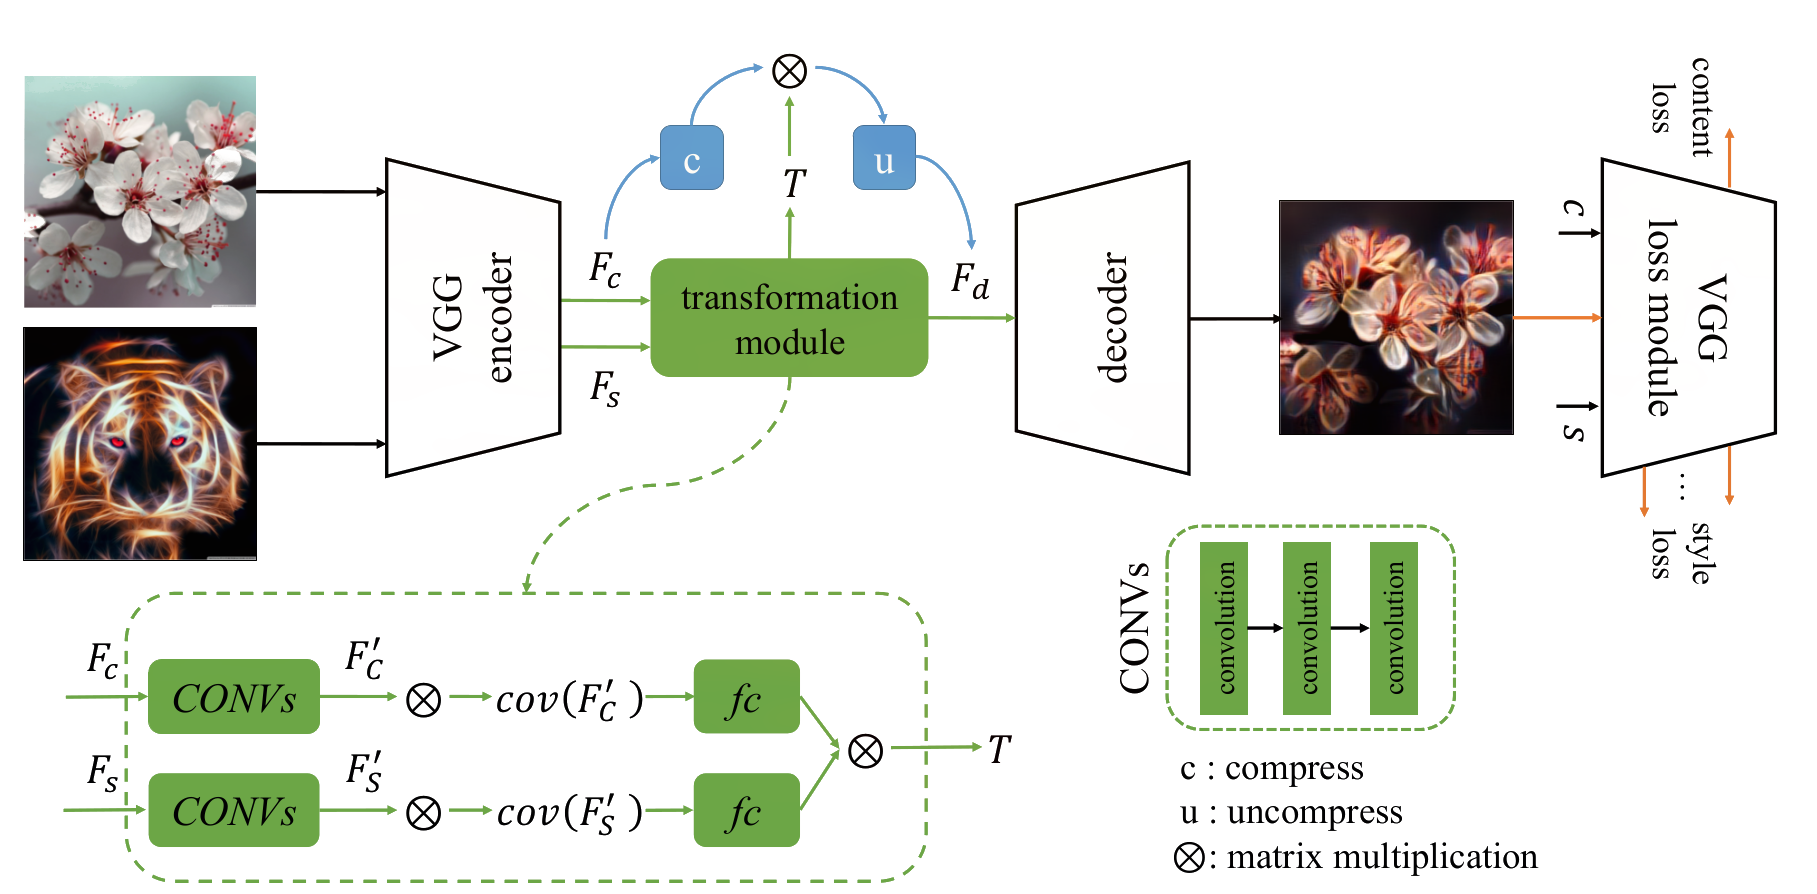
\includegraphics[scale=0.25]{overall_network.png}
        \caption{Overview of the network architecture}
        \label{fig:overall_network}
    \end{figure}
    
    
    \subsubsection{VGG} 
    \subsection{Transformation module}

\subsection{Pruning}
    \textbf{Filter pruning} 
    \textbf{Pruning schedule, datasets} 



\biblio % Needed for referencing to working when compiling individual subfiles - Do not remove
\end{document}
